
\begin{frame}{Udregn anbefalet hastighed}
Procedure
\begin{itemize}
\item 1. Udregn afstand til næste trafiklys
\item 2. Udregn grønne tidsrum
\item 3. Find signal, der kan nås
\item 4. Udregn og tilpas hastighed
\end{itemize}
\end{frame}

\begin{frame}{Udregn afstand til næste trafiklys}
Måles som euklidisk afstand mellem bilen og næste trafik lys.
\begin{itemize}
\item Der tages ikke højde for blokerende biler
\end{itemize}

Afstanden er $\infty$ hvis der ikke er flere trafiklys på ruten

Hvis afstanden er for stor, returneres fartgrænsen

\vspace{5mm}
\begin{center}
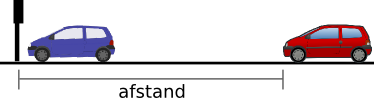
\includegraphics[width=0.8\textwidth]{../images/algdistance.png}
\end{center}
\end{frame}

\begin{frame}{Udregn grønne tidsrum}
\begin{center}
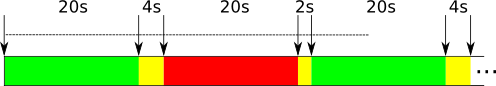
\includegraphics[width=1\textwidth]{../images/algphases4.png}
\vspace{5mm}
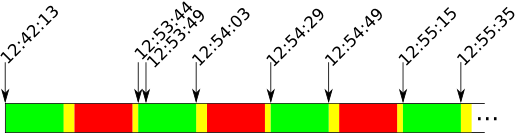
\includegraphics[width=1\textwidth]{../images/algphases5.png}
\end{center}
\end{frame}

\begin{frame}{Find signal, der kan nås}

Langsomste hastighed regnes som afstand over tid

\[\frac{\dist}{\tslow}\leq \velmax\]

Tager ikke højde for accelerationstiden
\begin{itemize}
\item I forvejen mange ukendte faktorer
\item Genberegner hvert sekund
\item Grænsetilfælde hvor et grønt signal godt kunne nås
\end{itemize}

\vspace{5mm}
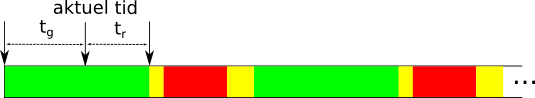
\includegraphics[width=1\textwidth]{../images/algphases1.png}

\end{frame}

\begin{frame}{Find signal, der kan nås, fortsat}
\begin{center}
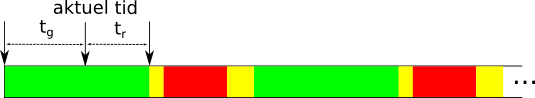
\includegraphics[width=1\textwidth]{../images/algphases1.png}
\vspace{5mm}
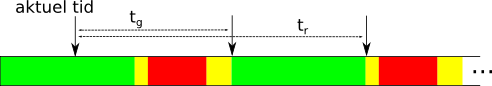
\includegraphics[width=1\textwidth]{../images/algphases2.png}
\vspace{5mm}
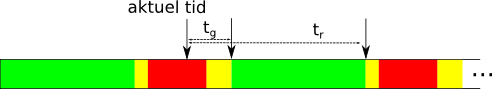
\includegraphics[width=1\textwidth]{../images/algphases3.png}
\end{center}
\end{frame}

\begin{frame}{Udregn hastighed og tilpas hastighed}
Anbefalet hastighed regnes som afstand over tid
\[\vel = \frac{\dist}{\tgreen}\]

Tilpas hastighed til øvre og nedre grænse
\begin{itemize}
\item Altid under fartgrænsen
\item Antager man ikke kan køre under 15 km/t
\end{itemize}

\end{frame}